%%%% ijcai25.tex

\typeout{IJCAI--25 Instructions for Authors}

% These are the instructions for authors for IJCAI-25.

\documentclass{article}
\pdfpagewidth=8.5in
\pdfpageheight=11in

% The file ijcai25.sty is a copy from ijcai22.sty
% The file ijcai22.sty is NOT the same as previous years'
\usepackage{ijcai25}

% Use the postscript times font!
\usepackage{times}
\usepackage{soul}
\usepackage{url}
\usepackage[hidelinks]{hyperref}
\usepackage[utf8]{inputenc}
\usepackage[small]{caption}
\usepackage{graphicx}
\usepackage{amsmath}
\usepackage{amsthm}
\usepackage{booktabs}
\usepackage{algorithm}
\usepackage{algorithmic}
\usepackage[switch]{lineno}
\usepackage{multirow}
\usepackage{amsmath,amssymb} 
\usepackage{comment}
\usepackage{xspace}
\usepackage{enumitem}
%\usepackage{hyperref}
\newtheorem{define}{Definition}
\newcommand{\attr}[1]{\textbf{#1}}
\newcommand{\rimsTool}{$\textsc{RIMS}{\mathsf{_{Tool}}}$\xspace}
\usepackage[dvipsnames]{xcolor} 
\newcommand{\rims}{$\textsc{RIMS}$\xspace}
\newcommand\btext[1]{{\color{blue}{#1}}}
\newcommand\rtext[1]{{\color{red}{#1}}}
\newcommand\massi[1]{{\color{orange}{#1}}}
%\usepackage{bbding}
\newcommand{\act}[1]{\textsf{\footnotesize #1}}
%
% These are recommended to typeset algorithms but not required. See the subsubsection on algorithms. Remove them if you don't have algorithms in your paper.
\newtheorem{proposition}{Proposition}
\newtheorem{definition}{Definition}

\usepackage{algorithm}
\usepackage{algorithmic}
\usepackage{xcolor} 
\usepackage{subfig}
\usepackage[table,xcdraw]{xcolor}

\usepackage{todonotes}

% Comment out this line in the camera-ready submission
%\linenumbers

\urlstyle{same}

% the following package is optional:
%\usepackage{latexsym}

% See https://www.overleaf.com/learn/latex/theorems_and_proofs
% for a nice explanation of how to define new theorems, but keep
% in mind that the amsthm package is already included in this
% template and that you must *not* alter the styling.
\newtheorem{example}{Example}
\newtheorem{theorem}{Theorem}
\newenvironment{proofsketch}{%
  \renewcommand{\proofname}{Proof Sketch}\proof}{\endproof}
% Following comment is from ijcai97-submit.tex:
% The preparation of these files was supported by Schlumberger Palo Alto
% Research, AT\&T Bell Laboratories, and Morgan Kaufmann Publishers.
% Shirley Jowell, of Morgan Kaufmann Publishers, and Peter F.
% Patel-Schneider, of AT\&T Bell Laboratories collaborated on their
% preparation.

% These instructions can be modified and used in other conferences as long
% as credit to the authors and supporting agencies is retained, this notice
% is not changed, and further modification or reuse is not restricted.
% Neither Shirley Jowell nor Peter F. Patel-Schneider can be listed as
% contacts for providing assistance without their prior permission.

% To use for other conferences, change references to files and the
% conference appropriate and use other authors, contacts, publishers, and
% organizations.
% Also change the deadline and address for returning papers and the length and
% page charge instructions.
% Put where the files are available in the appropriate places.


% PDF Info Is REQUIRED.

% Please leave this \pdfinfo block untouched both for the submission and
% Camera Ready Copy. Do not include Title and Author information in the pdfinfo section
\pdfinfo{
/TemplateVersion (IJCAI.2025.0)
}

\title{Proactive Data-driven Scheduling of Business Processes}

%%We acknowledge the support of the PNRR project FAIR - Future AI Research (PE00000013), under the NRRP MUR program funded by the NextGenerationEU, the HORIZON 2020 HumanE-AI project (Grant 952026)

% Multiple author syntax (remove the single-author syntax above and the \iffalse ... \fi here)

\author{
Francesca Meneghello$^{1,2}$
\and
Arik Senderovich$^3$ \and
Massimiliano Ronzani$^{1}$ \and
Chiara Di Francescomarino$^4$ \and
Chiara Ghidini$^5$\\
\affiliations
$^1$Fondazione Bruno Kessler, Via Sommarive, 18, POVO - 38123, Trento, Italy\\
$^2$Sapienza University of Rome, Via Ariosto, 25, 00185, Rome, Italy \\
$^3$York University, 4700 Keele St, Toronto,  ON M3J 1P3, Canada\\
$^4$University of Trento, Via Sommarive, 9, 38123 Trento, Italy\\
$^5$Free University of Bozen-Bolzano, via Bruno Buozzi, 1 - 39100, Bozen-Bolzano, Italy\\
\emails
\{fmeneghello, mronzani\}@fbk.eu,
sariks@yorku.ca,
c.difrancescomarino@unitn.it, chiara.ghidini@unibz.it
}


\begin{document}

\maketitle

\begin{abstract}
    Proactive scheduling creates 
robust offline schedules 
that optimize resource utilization and minimize job flow times. 
This work addresses scheduling challenges in business processes, often
encountered in service systems, 
which differ from traditional applications like manufacturing due to inherent uncertainties in activity durations, and human resource availability.
We model the business process scheduling 
problem (BPSP) as a variation of stochastic
resource-constrained multi-project scheduling (RCMPSP), and 
apply \emph{process mining} to infer unknown
parameter values from historical event data. To overcome 
the randomness in activity durations, we transform 
the problem into its deterministic counterpart, and 
prove that the latter provides a lower bound on the
Makespan of the stochastic problem. Our approach integrates data-driven Monte Carlo simulation with constraint programming to generate proactive schedules.
We evaluate our approach using synthetic datasets with varying levels of uncertainty and size.
In addition, we apply the approach to a real-world dataset from an outpatient cancer hospital, demonstrating its effectiveness in optimizing the process Makespan by an average of 5\% to 14\%.
\end{abstract}

\section{Introduction}
\label{sec:introduction}

We address the challenge of scheduling business processes in service domains such as finance (e.g., purchasing, order fulfillment), healthcare (e.g., patient flow management, appointment scheduling), and retail (e.g., order processing, supply chain coordination). Business processes are structured sets of activities that organizations execute to achieve various objectives, such as completing a sale, providing a service, or managing a supply chain~\cite{dumas2018fundamentals}. Unlike processes in manufacturing facilities, which typically involve predictable durations, and stable resource availability, business processes exhibit significant uncertainty and variability~\cite{shoush2022intervene,xu2016resource}. 
Specifically, scheduling business processes is notoriously complex due to the stochastic nature of activity durations caused by human behavior, as well as the time-varying availability of resources influenced by factors such as part-time schedules, overlapping responsibilities, and vacations. These challenges make traditional deterministic scheduling methods inadequate~\cite{pinedo2012scheduling}.

In response to this limitation, 
proactive scheduling techniques generate robust offline schedules~\cite{beck2007proactive,chaari2014scheduling}. These methods explicitly account for the stochastic nature of activity durations and aim to compute a \emph{proactive optimal solution} that achieves a pre-defined confidence level~\cite{beck2007proactive}. For example, a solution with a confidence level of \(1-\alpha\) ensures that the returned Makespan remains below an optimal threshold in at least (\(1-\alpha\)) of cases. While proactive scheduling has made significant progress in addressing variability through probabilistic activity durations~\cite{satic2022performance,liu2020multi,hauder2020resource,chen2019research,beck2007proactive}, critical gaps remain. Notably, the challenge of \emph{planned} resource unavailability is seldom addressed. Although studies incorporate the planned unavailability of resources, some overlook the uncertainty of duration~\cite{kreter2018mixed}, while others fail to handle the complexity and variability typical of business processes~\cite{yang2020multi,winklehner2022flexible}.

Beyond methodological gaps, many real-world business processes face an additional practical challenge: the lack of readily available data on key scheduling parameters. Information such as activity durations, their probabilistic distributions, and resource availability calendars is often incomplete or missing. Without access to this data, even advanced scheduling techniques struggle to perform effectively in real-world settings. To bridge this gap, we employ \emph{process mining}, a data-driven approach designed to extract knowledge and insights from event logs~\cite{van2016data}. Event logs are datasets that document process executions, capturing details such as activity types, start and end times, and the resources assigned to each activity. 

Building on this foundation, we formulate the Business Process Scheduling Problem (BPSP) and establish its relationship to the well-known Resource-Constrained Project Scheduling Problems (RCPSP). Our approach leverages both process mining and proactive scheduling methods to tackle both the inherent uncertainty in
business processes, and lack of knowledge of the problem. Specifically, we develop a framework that combines data-driven simulation~\cite{MeneghelloFGR25}, and constraint programming~\cite{kreter2018mixed}: we construct a constraint programming model that generates deterministic schedules for the BPSP, verify them using the simulator, and select the best performing schedules. These schedules are evaluated and optimized to minimize the uncertain Makespan while achieving a pre-specified confidence level, ensuring robustness against variability and resource constraints.

We evaluate our approach in two phases 
to demonstrate both its effectiveness and applicability. In the first phase, we conduct experiments using synthetic data, allowing us to systematically test the framework’s ability to handle varying levels of uncertainty while accounting for resource calendars. This controlled environment ensures that the method can adapt to diverse scheduling scenarios and reliably optimize outcomes under uncertainty. 
In the second phase, we validate the applicability of our approach by applying it to real-world event logs from a healthcare process, achieving an optimization of the process Makespan by an average of 5\% to 14\%.
Using process mining techniques, we extract BPSP parameters from the logs and employ our framework to generate optimal schedules. This highlights the practical value of our method, showcasing its ability to address complex, data-driven scheduling challenges in a real-world domain.


%To summarize, the main contributions of our work are:
%\begin{itemize} 
%\item We formulate the Business Process Scheduling Problem (BPSP) to address the challenges of scheduling processes with stochastic activity durations, and planned resource unavailability. 
%\item We propose a novel BPSP solution framework that combines data-driven business process simulation, leveraging event logs and process mining, with constraint programming to generate robust and optimized schedules under uncertainty. 
%\item We evaluate our framework using synthetic benchmarks and real-world event logs from the healthcare domain. 
%\end{itemize}


\section{Business Process Scheduling}
\label{sec:motivating}
\begin{figure*}[t]
    \centering
    \subfloat[\centering BPMN\label{fig:TPN}]{{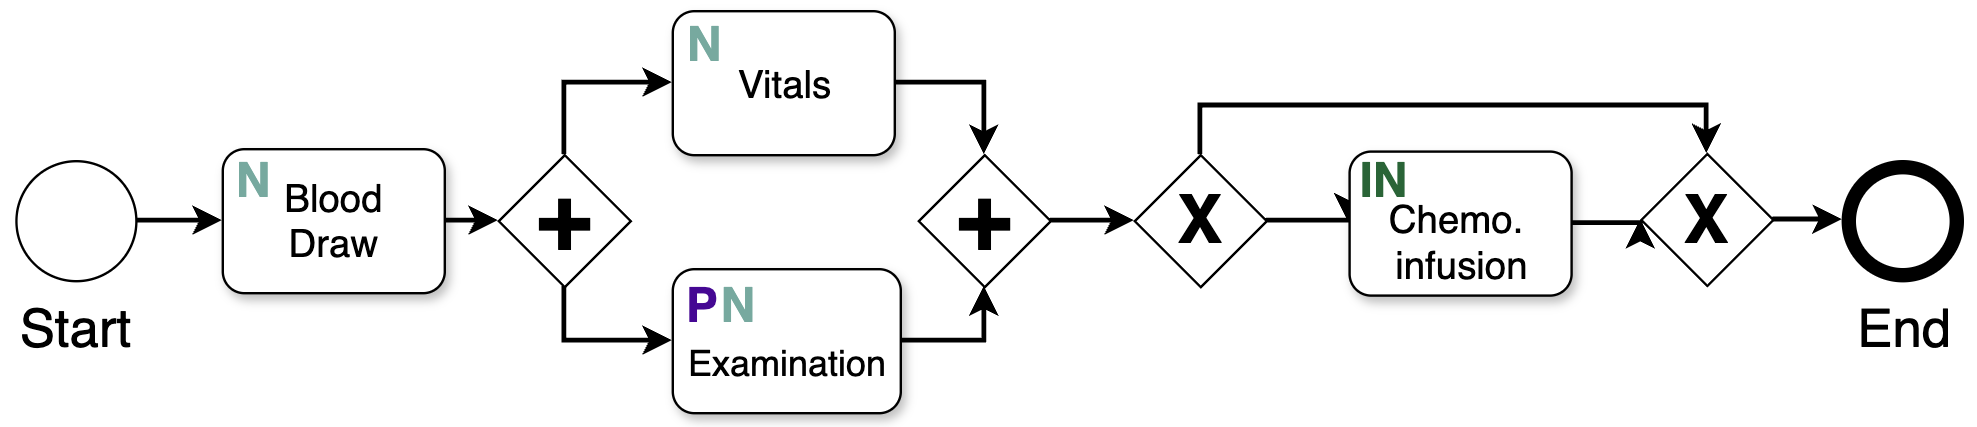
\includegraphics[width=0.75\textwidth]{images/bpmn.png} }}%
    \qquad
    \subfloat[\centering Resource calendars\label{fig:calendar}]{{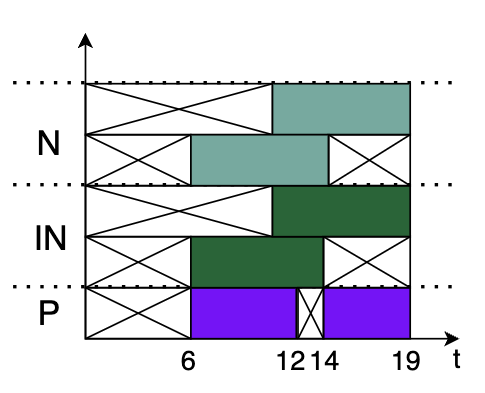
\includegraphics[width=0.20\textwidth]{images/calendars.png} }}%
    \caption{Running example of hospital process}%
    \label{fig:running_example}%
\end{figure*}
In this part, 
we first motivate our work with a real-life hospital
example. Then, we proceed to define the business
process scheduling problem (BPSP),
and lastly,
discuss the use of process mining for inference of BPSP parameters
from data.


\subsection{Motivating Example} We are motivated
by a hospital process 
that provides a sequence of treatments to cancer patients. 
The resources involved in the process, nurses (\act{N}), physicians (\act{P}), 
and infusion nurses (\act{IN}), are shared among patients 
and must be scheduled ahead of time. 
The duration of treatments varies significantly based on patient-specific context (e.g., patient complexity). 
Furthermore, the resources involved are not always available, as they follow specific shift schedules
and may go on planned vacations. For instance, 
nurses work 8 hours a day, 5 days a week, either in the morning or in the afternoon. Physician calendars are
highly variable, and depend on exogenous factors 
(e.g., physicians serving in multiple hospitals). 




The hospital process is depicted in Figure~\ref{fig:TPN}, which illustrates possible patient pathways. The activities are represented by white rectangles, and the time required to complete each activity is defined by probability distribution functions. The process begins with the \act{Blood Draw} activity, performed by a nurse (\act{N}), and continues with the parallel execution of the \act{Vitals} (for vital signs) and \act{Examination} activities, performed by a nurse and a physician (\act{P}), respectively. Finally, based on previous activities, the physician decides whether to proceed with \act{Chemo. Infusion}.

To complement the picture, Figure~\ref{fig:calendar} illustrates resource shifts for a typical day. Nurses have various shifts, which overlap for only two hours, between \act{11 am} and \act{2 pm}, while the physician has a two-hour break during which no \act{ examination} activity can be performed. The hospital processes approximately 1000 patients per day, involving over 5000 activities. The goal is to find a proactive schedule that probabilistically minimizes the global Makespan, e.g., the time that the last patient leaves cannot exceed \act{6PM} with probability of at least $0.95$. 

\subsection{Problem Definition} 
Referring to the definition in ~\cite{sanchez2023survey}, a case in a business process corresponds to a project, and the activities within the case map to the jobs that comprise the project. Business process scheduling problems (BPSPs) can therefore be represented using the following parameters\footnote{RCMPSP notation taken from~\cite{sanchez2023survey}.}: 
\begin{itemize}
    \item $\mathcal{I}$ is the set of cases enumerated by $i \in \{1, 2,....|\mathcal{I}|\}$,
    \item $A_i  = \{a_1, \ldots, a_{|A_i|}\}$ is the set of activities comprising case $i$, where $a_j, a_k$ may correspond to the same activity type (e.g., examination),
    and may repeat within a case,
    \item $\mathcal{A}$ is the set of all possible activity types, and $\phi$ is a mapping from activities to their types, $\phi(a_j) \in \mathcal{A}$,
    \item $\Pi_{i,a_j} \subseteq A_i$ represents activities that precede activity $a_j \in A_i$, i.e., their completion precedes the start of $a_j$,
    \item $\mathcal{R}$ is the set of resources involved in the process, with $r \in \{1, 2,....|\mathcal{R}|\}$, and
     $C_r$ being the capacity of $r$,
    \item $R_{i,a_j} \subseteq \mathcal{R}$ are the resources required to perform activity $a_j$ in case $i$, and $\rho(a_j) = R_{i,a_j}$ is a function that returns the set of resources required by an activity,
    \item $\mathcal{T} = \{0, 1, \ldots, T\}$ is a set of time periods (e.g., minutes) during a scheduling horizon of length $T$,
    \item $D_{i,a_j} \sim \mathcal{P}_{i,\phi(a_j), \rho(a_j)}$ is the number of time periods required to perform activity $a_j$ in case $i$, which follows the probability distribution $\mathcal{P}$ that depends on case $i$, activity type $\phi(a_j)$ and set of resources $\rho(a_j)$.\footnote{ The only stochastic components of BPSP are activity durations.}
    %$D_{i,a_j} \sim \mathcal{P}_{i,\phi(a_j), \rho(a_j)}$ is the (resource-, case- and activity type-dependent) \emph{random} number of time periods required to perform activity $a_j$ in case $i$, with $\mathcal{P}_{i,\phi(a_j), \rho(a_j)}$ being the distribution of the duration.\footnote{ The only stochastic components of BPSP are activity durations.} 
    \item $v_{r,t} \in \{0,1\}$ is the resource availability calendar, which is $1$ if resource $r$ is available at time period $t \in \mathcal{T}$.
\end{itemize} 
It is worth mentioning that the BPSP is a variation of the RCPSP that, 
to the best of our knowledge, has not yet been addressed in the scheduling literature~\cite{sanchez2023survey}.

Scheduling the business process is to assign each activity $a_j \in A_i,\ i=1,\ldots, |\mathcal{I}|,\ j=1,\ldots,|A_i|$ with a start time. Resource assignment is defined based on the activity requirement $R_{i,a_j}$, where non-interchangeable resources are treated as distinct.
%(resource assignment is implicit from the activity requirement $R_{i,a_j}$). 
Optimal scheduling in our setting is to find a schedule such that the 
latest completion time 
among all cases, i.e., the global Makespan $M$, is minimized. 



\begin{table}[t]
\resizebox{0.90\columnwidth}{!}{
    \begin{tabular}{c c c c c}
        \toprule
        \textbf{CaseId} & \textbf{Activity type}  & \textbf{Start} & \textbf{Complete} & \textbf{Resources} \\ 
        \midrule
        \act{1} & \act{Blood Draw} & \act{08:00} & \act{08:06} & \attr{N} \\
        \act{2} & \act{Blood Draw} & \act{08:01} & \act{08:07} & \attr{N} \\
        \act{3} & \act{Blood Draw} & \act{08:01} & \act{08:05} & \attr{N} \\
        \act{3} & \act{Vitals} & \act{08:05} & \act{08:11} & \attr{N} \\
        \act{2} & \act{Examination} & \act{08:07} & \act{08:14} & \attr{P} \\
        \act{2} & \act{Vitals} & \act{08:10} & \act{08:14} & \attr{N} \\
        \act{3} & \act{Examination} & \act{08:10} & \act{08:25} & \attr{P,N} \\
        \act{1} & \act{Vitals} & \act{08:11} & \act{08:14} & \attr{N} \\
        \act{1} & \act{Examination} & \act{08:11} & \act{08:30} & \attr{P,N} \\
        \act{2} & \act{Chemo. Infusion} & \act{08:20} & \act{09:10} & \attr{IN} \\
        \act{1} & \act{Chemo. Infusion} & \act{08:30} & \act{09:40} & \attr{IN} \\
        \bottomrule
    \end{tabular}
}
\caption{Example of a simple event log.}
\label{table:real_log_DT}
\end{table}



\subsection{Learning BPSP Parameters From Event Logs} 
If all parameters of the BPSP are at hand, one can immediately switch to solving the underlying problem.
However, if this is not the case, one can use historical data to infer these parameters with the use 
of process mining methods. 

Process Mining~\cite{van2016data} integrates data science with business process analysis to extract insights from event logs recorded by enterprise information systems, such as EPIC in healthcare~\cite{johnson2016comprehensive}. Event logs (see Table~\ref{table:real_log_DT}) provide a valuable source of data for learning the parameters required for scheduling problems. 
An event log consists of multiple cases, where each case 
is a sequence of events 
corresponding to the execution of a case, e.g., a single journey of a patient in a hospital. Each event 
in the sequence is a measurement of an activity and its characteristics. 
Specifically, events capture the type of activity, the resources involved and the start and end timestamps that define the duration of the activity.


\paragraph{Learning Activities and Precedence.} Activity types, which represent categories of activities performed in the process, are determined from the labels of activities recorded in the event log. Mapping these observed activities to predefined types involves grouping activities based on domain knowledge or textual similarity. The durations of activities can be derived from the start and end timestamps recorded in the event log. By analyzing these timestamps, probability distributions can be fitted to the observed durations of each activity type, such as normal or log-normal distributions, depending on the observed data, c.f.,~\cite{simod}. Precedence constraints can be inferred by examining the sequential order of activities in traces, identifying dependencies between activities where the completion of one activity consistently precedes the start of another~\cite{senderovich2019learning}. 

\paragraph{Inferring Resources and Capacities.} Resource capacities can be inferred by analyzing the frequency of resource usage over time, leveraging approaches such as \textit{SchedMiner}~\cite{SenderovichRGMM15}. 
The effective capacity is estimated by considering the maximum resource utilization observed in the event log. This estimate often serves as a tight lower bound, as there remains a small probability that some resources were available but never utilized.

%By determining peak resource utilization, capacity estimates act as lower bounds when full utilization is not observed in the log. 
Resource availability calendars can be constructed by analyzing the distribution of timestamps associated with resource usage, identifying periodic patterns such as daily or weekly schedules, which can be assumed constant over extended 
periods. Resource requirements for activities can be extracted from the resource identifiers associated with events in the log. 


\paragraph{Threats to Validity.} The application of process mining techniques relies on several assumptions. It is assumed that logs are complete, capturing all resources and activities involved in the process, and that activities are non-preemptive, meaning they run to completion once started. Resource capacities are assumed to remain fixed over time, with resources becoming available immediately after completing an activity, unless they are absent according to their calendar. Additionally, activity durations are assumed to follow a known distribution, and resource calendars are considered periodic and consistent over the given time horizon. All of these assumptions may be violated in practice. 

A first step in addressing threats to validity in process mining is to use representative event logs, i.e., logs that cover a time period meaningful to the process life-cycle and minimize the variability caused by seasonal behaviors. Variability in resource capacities and behaviors can be mitigated by estimating the capacity of pools of resources performing shared activities. Hence, resource pools reflect average performances and are not influenced by the behavior of individual resources. Finally, with respect to the
time perspective of the process, many state-of-the-art approaches replace predefined distributions with advanced statistical or machine learning models to more accurately capture process dynamics.






\section{Proactive BPSP}
\label{sec:method}

\begin{figure*}[t]
\centering
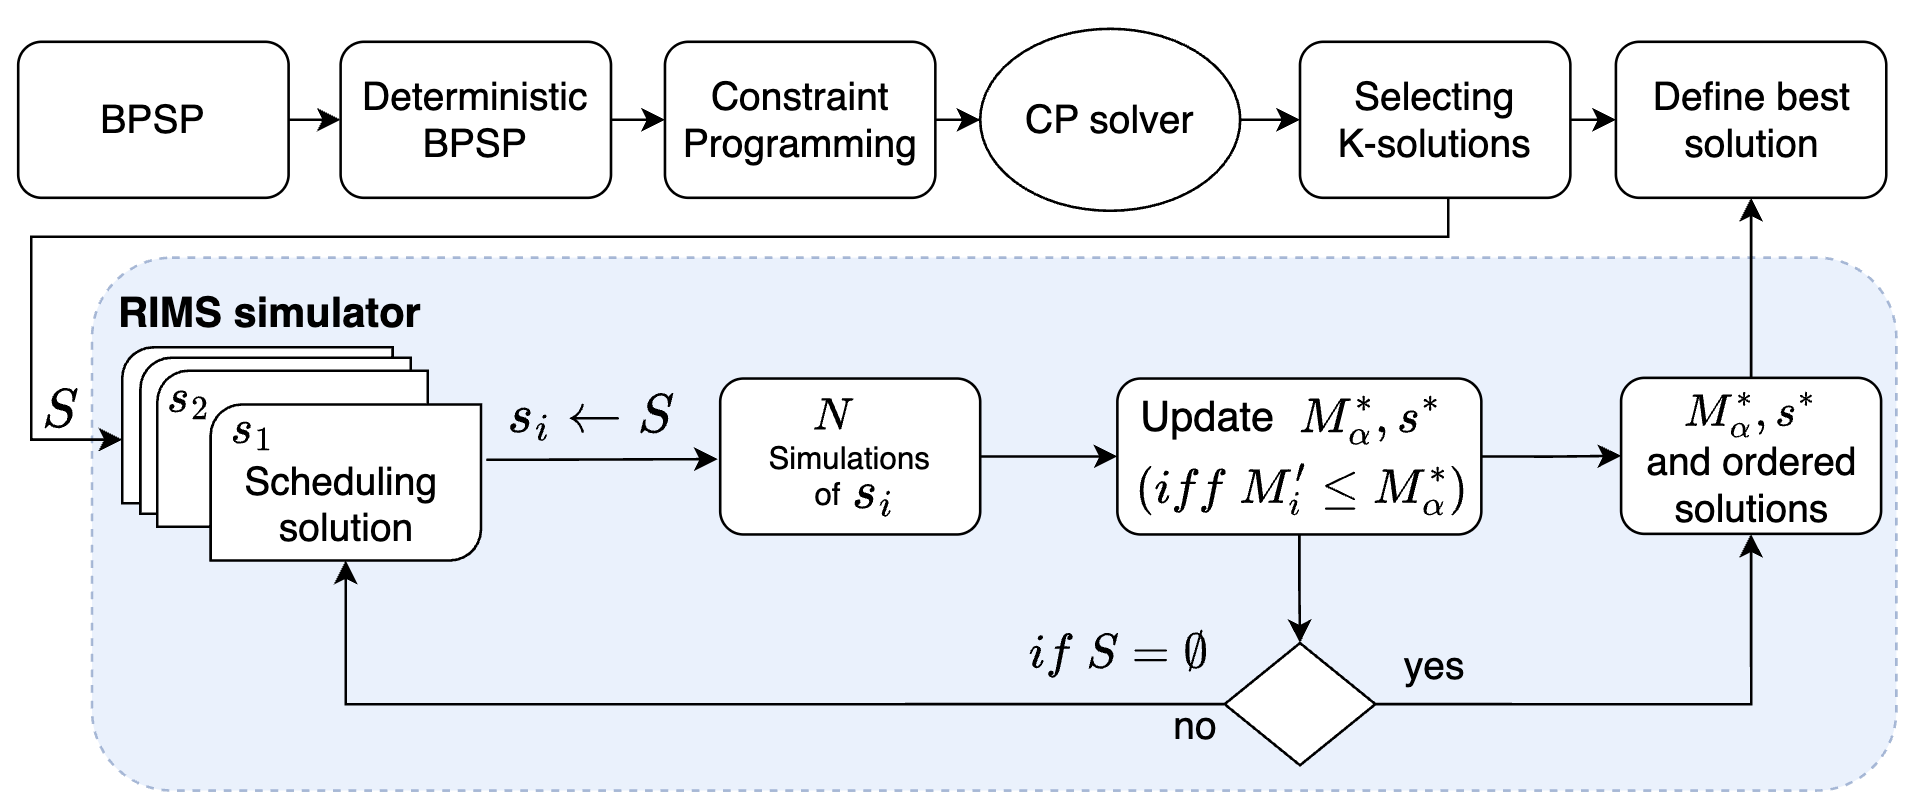
\includegraphics[width=0.6\textwidth]{images/pipeline_rims3.png}
\caption{Our approach to Proactive Business Process Scheduling.}
\label{fig:pipeline}
\end{figure*}
Figure~\ref{fig:pipeline} illustrates the steps of our method. First, we define the BPSP based on either prior knowledge or by estimating its parameters from data.
To manage the stochastic activity durations, we convert the stochastic BPSP into its deterministic counterpart by employing the transformation proposed in~\cite{beck2007proactive}, which is described in the next Section.
Next, once the problem becomes deterministic, we construct a Constraint Programming (CP) model, and a CP solver is employed to obtain solutions that iteratively minimize the global Makespan $M$ until either an optimal deterministic solution is found, or a time limit is reached. Once CP solutions are obtained, we first select the \emph{top-$K$} solutions. Finally we employ Monte-Carlo simulation to identify the best solution. Below, we detail the different steps, and justify our design choices.


\subsection{From Stochastic to Deterministic BPSP}
\label{sec:stoc_to_det}

The activity durations in a BPSP are random. Therefore, minimizing 
the Makespan
implies
finding the smallest possible value of $M^*_\alpha$ such that a solution exists with a random Makespan that, with high probability, $1-\alpha$ is less than $M^*_\alpha$. We refer to $M^*_\alpha$ as the probabilistically minimum Makespan.

To transform the BPSP into a deterministic problem, we use the approach proposed by~\cite{beck2007proactive}, which associates a deterministic problem with the probabilistic one by transforming each random duration into the sum of its mean value and a buffer that depends on its standard deviation. More formally, for activity $a_j$ in case $i$, the deterministic duration
that is associated with it is, \begin{equation}
d_{i,a_j} = \mu_{i, a_j} + q \cdot \sigma_{i, a_j},\label{eq:duration}
\end{equation} with 
$\mu_{i, a_j}$ being the mean duration
of the activity, $\sigma_{i, a_j}$ being its standard deviation
and $q\geq0$ being
an uncertainty coefficient that provides a buffer for the mean value.\footnote{Note that we assume the existence of the first two moments of the distribution for activity durations.}
If $q=0$, the mean value is used as activity duration across the board.
All other components of the problem are deterministic, 
and remain unchanged. 
%The approach is grounded in theory, which we lay out, and extend in the following part.
The challenge with the transformation defined in \eqref{eq:duration} is the identification of the value of a value of $q$ such that the makespan $M_q$ of the deterministic problem serves as a lower bound for the makespan $M_\alpha$ of the stochastic problem. In the remaining of the Section we provide some details on the solution proposed in~\cite{beck2007proactive} and summarized the value of $q$ defined in \eqref{eq:qU}.


\subsubsection{Lower-Bound Guarantees for BPSP} 


The work in~\cite{beck2007proactive} shows that for Resource-Constrained Project Scheduling Problem (RCPSP),
a lower bound for the probabilistic Makespan $M^*_\alpha$ is provided by the makespan $M_U$ given by the solution of the deterministic problem obtained using the transformation \eqref{eq:duration} with the value of  $q$ set to
\begin{equation}
q_U = \frac{\Phi^{-1}(1-\alpha)}{\sqrt{U}},
\label{eq:qU}
\end{equation}
where $\Phi^{-1}$ is the inverse of the standard normal cumulative distribution function (CDF), and $U$ represents an upper bound on the number of uncertain activities along the deterministic critical path (e.g., $U$ can be set to the total number of activities).
Furthermore, the authors in~\cite{beck2007proactive} demonstrate that this lower bound can be tightened by selecting different values for \( q \) when additional assumptions are satisfied. The lower bound result is critical to efficiently select models using Monte Carlo simulation.


However, to apply the result in the BPSP case, we must overcome three violations of the classical RCPSP assumptions, namely multiple cases, potentially inter-dependent activity durations, and planned resource unavailability. 
The first two violations are straightforward to address.  
Since we consider the Makespan with respect to the latest activity regardless of the case, one can view BPSP as a single-case scheduling problem~\cite{sanchez2023survey}.  
Moreover, when conditioning on the case, the resources, and the activity being processed, activity durations become independent of each other. This property, referred to as conditional independence, ensures that the result from~\cite{beck2007proactive} applies, as we assume the case identifier and activity information (i.e., its type and required resource set) are known.  

The only significant limitation that remains unresolved relates to resource calendars.
To prove that $q_U$ indeed yields a lower-bound we must
first define so-called \emph{positive precedence expressions}.
The set $E$ is a set of precedence constraints between activities $a_i$ and $a_j$ specified as $\texttt{before}(i, j)$, i.e., the constraint that activity $a_j$ cannot 
start earlier than the completion of $a_i$.
%For activities $a_i$ and $a_j$, the expression $\texttt{before}(i, j)$ represents the constraint that activity $a_j$ cannot start earlier than the completion of $a_i$. 
We are now ready to define positive precedence expressions (PPEs). 

\begin{definition}[Positive Precedence Expressions (PPE)]
\label{def:ppe} 
The set $E$ is referred to as a positive precedence expressions over a set of activities $A$ if it is the smallest set satisfying:
\begin{enumerate}
    \item $ \forall a_i, a_j, \texttt{before}(i, j) \in E$.
    \item If $\phi, \psi \in E$, then $\phi \wedge \psi \in E$ and $\phi \vee \psi \in E$.
\end{enumerate}
\end{definition} In~\cite{beck2007proactive} it is 
shown that for scheduling problems that 
can be written as a conjunction of PPEs,
the proposed transformation that uses $q_U$ (as above) provides a lower-bound
on the stochastic problem. Therefore,
what remains to be shown is that BPSP can be expressed 
by a conjunction of PPEs.
\begin{proposition}
Selecting $q= q_U$ yields a lower-bound solution to the stochastic BPSP. \label{prop:lower}
\end{proposition}
\begin{proof}
We build the proof on the result of~\cite{beck2007proactive}, who established a lower bound for RCPSPs that do not account for resource unavailability. We will treat resource `vacations'
as dummy activities that we must schedule in addition to the other activities. The core argument relies on the ability to represent RCPSP constraints as Positive Precedence Expressions (PPEs).
Specifically, the constraints of an RCPSP can be expressed as a conjunction of PPEs~(\cite{beck2007proactive}):
\begin{enumerate}
    \item \textbf{Precedence Constraints (\( \phi \))}: Precedence relationships between activities \( a_i \) and \( a_j \) are represented as primitive precedence expressions \( \texttt{before}(i, j) \). Let \( \phi \) denote the conjunction of all such precedence constraints.

    \item \textbf{Resource Constraints (\( \psi \))}: Resource constraints can be represented using forbidden sets. A forbidden set \( H \subseteq \mathcal{A} \) consists of activities whose simultaneous execution exceeds the capacity of a resource \( r \), $C_r$. Resource constraints are satisfied if, for all \( H \in F \), there exist two activities \( a_i, a_j \in H \) such that \( \texttt{before}(i, j) \) holds. This is expressed as:
    \[
    \psi = \bigwedge_{H \in F} \bigvee_{a_i, a_j \in H, i \neq j} \texttt{before}(i, j).
    \]
\end{enumerate} Combining these, the constraints of an RCPSP are represented as \( \phi \wedge \psi \), which is a conjunction of PPEs. In BPSP, resource unavailability introduces additional constraints:
each resource \( r \) has an availability calendar \( v_{r,t} \), where \( v_{r,t} = 1 \) if \( r \) is available at time \( t \), and \( 0 \) otherwise.
To incorporate resource unavailability, we redefine and extend the notion of forbidden sets:
\begin{enumerate}
    \item Capacity forbidden sets \( H \) are defined as in RCPSPs, representing sets of activities whose simultaneous execution exceeds the capacity of a resource \( r \).
    \item For resource unavailability, we extend \(H\) with additional constraints for each resource \( r \) and time \( t \) where \( v_{r,t} = 0 \). The extended forbidden sets, denoted $H'$, ensure that no activities requiring \( r \) overlap during unavailable periods.
\end{enumerate} The resource constraints with unavailability can then be expressed as:
\[
\psi_u = \bigwedge_{H' \in F'} \bigvee_{a_i, a_j \in H', i \neq j} \texttt{before}(i, j),
\]
where \( F' \) is the extended set of forbidden sets that includes both capacity constraints and unavailability constraints.

The combined constraints for BPSP, including resource unavailability, can now be expressed as:
\[
\phi \wedge \psi_u,
\]
where \( \phi \) represents precedence constraints, and \( \psi_u \) represents resource constraints, including unavailability. Each component is a conjunction of PPEs, ensuring that the overall problem retains the PPE structure.

Since BPSP constraints can be expressed as a conjunction of PPEs, the results from~\cite{beck2007proactive} apply, and \( q_U \) provides a lower bound on the stochastic Makespan.

\end{proof} 


% \begin{proofsketch}
% This proof builds on~\cite{beck2007proactive}, who showed that Resource-Constrained Project Scheduling Problem (RCPSP) constraints can be expressed as a conjunction of Positive Precedence Expressions (PPEs). Precedence constraints (\( \phi \)) are primitive expressions \( \texttt{before}(i, j) \), and resource constraints (\( \psi \)) are modeled using forbidden sets, ensuring no subset of activities requiring the same resource exceeds its capacity. Together, RCPSP constraints form \( \phi \wedge \psi \), retaining the PPE structure.


% To handle resource unavailability in the BPSP, forbidden sets are extended. For each resource \( r \) and time \( t \) where \( v_{r,t} = 0 \), additional constraints ensure that activities requiring \( r \) do not overlap during unavailable periods. These extended forbidden sets, \( H' \), combine capacity and unavailability constraints, forming \( \psi_u \). The BPSP constraints are then expressed as \( \phi \wedge \psi_u \), preserving the PPE structure. \btext{In essence, unavailability periods are injected as `dummy' activities that must be considered when scheduling.} 

% Since BPSP constraints remain a conjunction of PPEs, the results reported in~\cite{beck2007proactive} apply directly. Thus, \( q_U \), a lower bound for RCPSPs, extends as a valid lower bound on the stochastic Makespan of BPSPs, even with resource unavailability.\footnote{Full proof is available in the supplementary material.}
% \end{proofsketch}

%We shall use this result in the 
%last part of our approach where we select 
%stochastic candidates based on deterministic solutions and Monte-Carlo %simulation.



%\textit{Evaluating a solution of a probabilistic RCMSPS can be done by using Monte Carlo Simulation: for each of a large number of trials we randomly sample the durations of every activity and generate the makespan associated with that trial}. We fix $\alpha$ to bound the probabilities and we assume a value in range $(0, 0.05]$.

\subsection{Solving Deterministic BPSP with CP}

%We use a common formalism to model RCPSP problems that involve optional activities and alternative resources~\cite{baptiste2001constraint,liu2019robust,ari}, and .
In this section, we present a CP model of the 
deterministic BPSP. We use the general CP model
proposed by \cite{senderovich2019learning}, 
and extend it with the planned unavailability~\cite{hauder2020resource}.

In particular, we employ the optional interval variable, $var$, to effectively represent the activities in our deterministic BPSP. The presence, start time, and duration are represented by \act{Pres}($var$), \act{Start}($var$) and 
\act{Length}($var$), respectively, with \act{Pres}($var$)~$=0$ indicating
its absence in the constraint model.
For each activity, $a_j \in A_i$, to be executed in a case $i$ we define an interval variable $x_{i,a_{j}}$ where~\act{Start}($x_{i,a_{j}}$)~$\geq 0$ and~\act{Pres}($x_{i,a_{j}}$)~$= 1$. The precedence relations between the activities in $i$ are guaranteed by the form \act{EndBeforeStart}~($x_{i,a_{k}},x_{i,a_{j}})$ $ \forall a_k \in \Pi_{i,a_j}$, ensuring that \act{Start}($x_{i,a_{j}}$) $\geq$ \act{Start}($x_{i,a_{k}}$) $+$ \act{Length}($x_{i,a_{k}}$). %Each activity can be performed by exactly one resource respecting its planned unavailability. 
To represent the resources assignments we define, $$X_{a_j}~=\{\overline{x}_{i,a_j,R}: d_{i,a_j},R \subseteq \mathcal{R}\},$$ as set of optional interval variables, where $\overline{x}_{i,a_j,R}$ represents the activity $a_{j} \in A_i$ assigned to a set of resources $R \subseteq \mathcal{R}$ with duration \act{Length}($\overline{x}_{i,a_j,R}$)$= d_{i,a_j}$ defined as~\eqref{eq:duration}.

%where $\overline{x}_{i,a_j,r}$ represents the activity $a_{j} \in A_i$ assigned to resource $r \in \mathcal{R}$ with duration \act{Length}($\overline{x}_{i,a_j,r}$)$= d_{i,a_j}$ defined as~\eqref{eq:duration}. 

\act{Alternative}(${x}_{i,a_j}, X_{a_j}$) ensures that only one interval variable from $X_{a_j}$ is present, and it starts and ends together with ${x}_{i,a_j}$. \act{Unavailable}($\overline{x}_{i,a_j,r}, v_{r,t}$) guarantees that the start and end times of the activity overlap with an available period in the resource calendar, $v_{r,t}$.
Finally, to ensure that the total number of present and executing activity interval variables assigned to a resource does not exceed its capacity, we define \act{Cumulative}($\{\overline{x}_{i,a_j,r}: a_j \in A_i \}, C_r$), $\forall r \in \mathcal{R} \; \text{and} \; \forall i \in \mathcal{I}$.

The goal is to minimize the global Makespan, i.e., the maximum end time across all activities.
\[
\text{Makespan} = \max_{i \in \mathcal{I}, a_j \in A_i} \text{\act{Start}}(x_{i,a_j}) + \act{Length}(x_{i,a_j})
\]




\subsection{Solution Selection \& Monte Carlo Simulation}

In this phase, we apply a CP solver\footnote{We use the Python version of Google OR-Tools (v9.11.4210) as our CP solver.} to
collect feasible solutions that iteratively minimize 
the global Makespan until either the optimal solution is found or a pre-defined time limit is reached. 
To evaluate the solutions returned by the CP solver and we employ Monte Carlo Simulation to select, $M_\alpha^*$, the one that yields the probabilistic minimum Makespan. 
%-- i.e., a solution that, with high probability $1 -\alpha$ guarantees a Makespan lower than $M^*_{\alpha}$ -- we employ Monte Carlo simulation. 
$M_\alpha^*$ is defined as the 
$
M_\alpha^* = \min_{s_i \in S} M'_{s_i}
$
where $M'_{s_i}$ represents the $100(1 - \alpha)$th percentile of Makespan
values computed over $N$ Monte Carlo simulations of a solution $s_i$ returned by the CP solver.
Each Makespan value, corresponds to the maximum end time across all activities in the simulation

Firstly, we select a subset of $k$-solutions from those returned by the solver, leveraging the 
well-established correlation between deterministic and probabilistic solutions~\cite{BonfiettiLM14}.\footnote{The evaluation section provides a detailed explanation of the $k$-solutions selection process.} 
Then, we iteratively evaluate selected solutions by performing a large number of independent simulations using the original stochastic activity durations to identify $M^*_{\alpha}$.  



\section{Evaluation}
\label{sec:evaluation}

%In this section, we present the experimental settings, and the two experiments,
%based on synthetic and real-world datasets, that we used to assess our methodology.


\begin{figure*}[t]
    \centering
    \subfloat[\centering Definition of Deterministic BPSP with $q_U$\label{fig:calendar_qU}]{{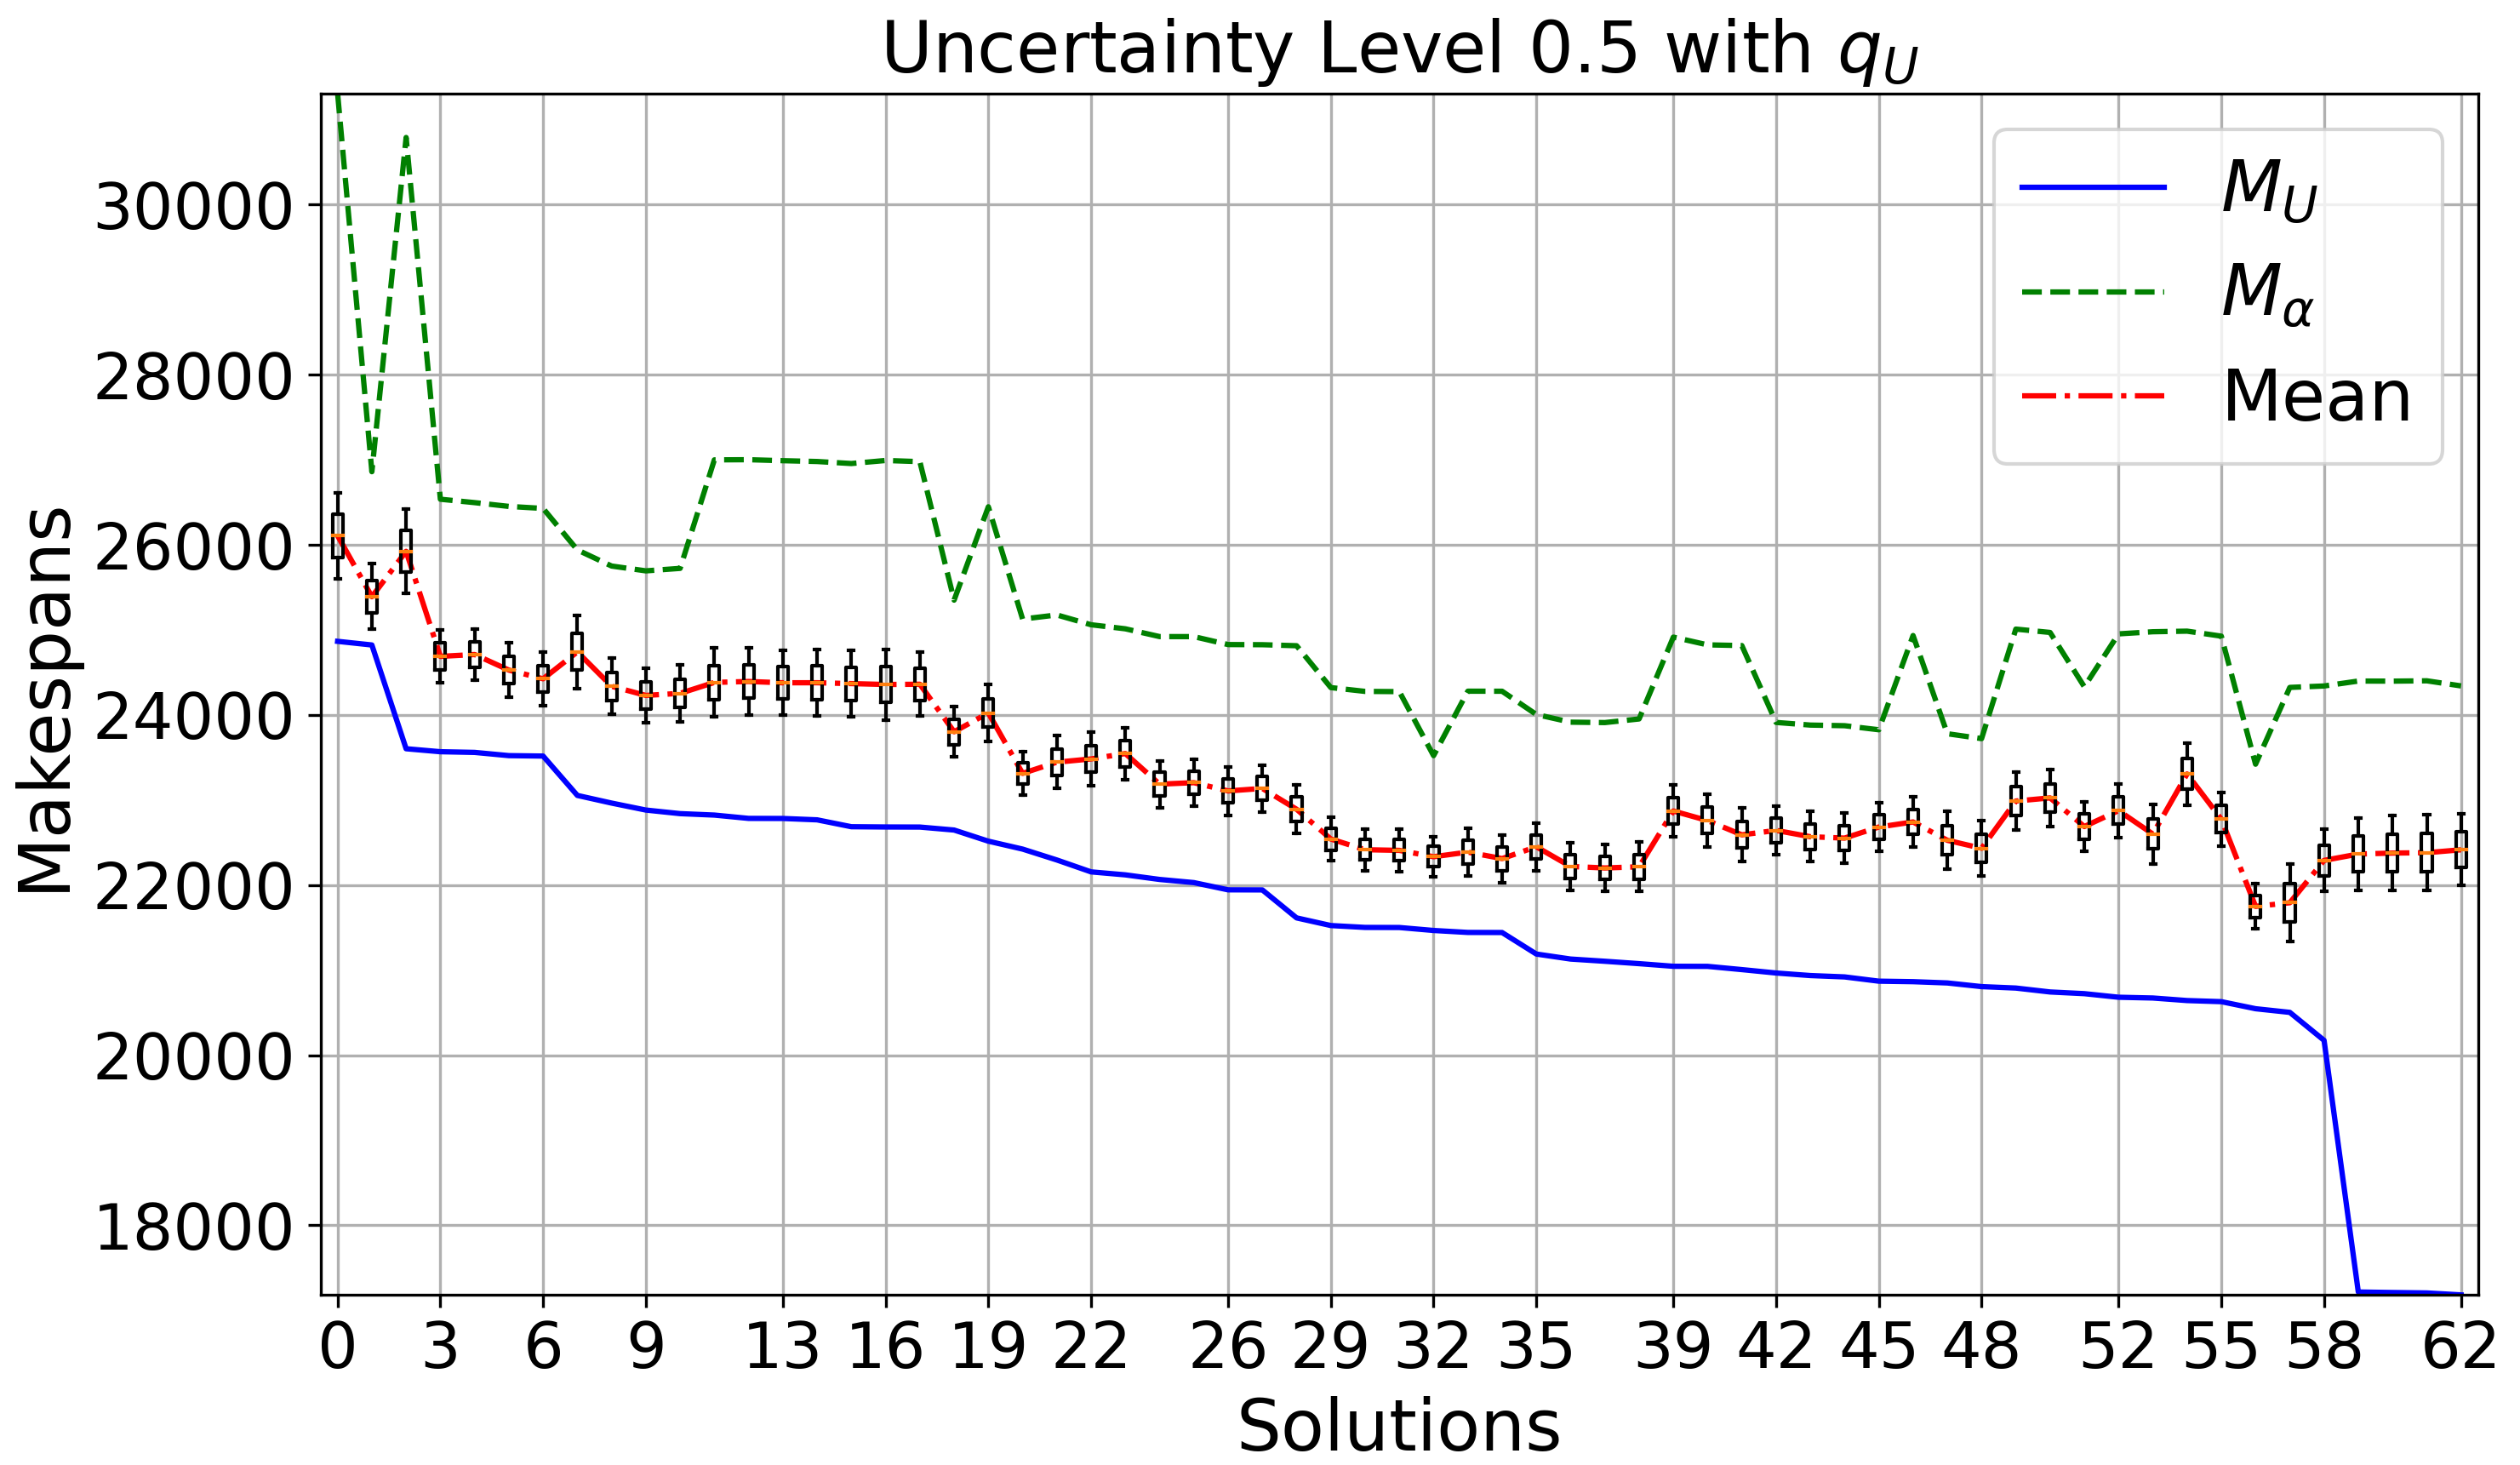
\includegraphics[width=0.47\textwidth]{images/uncertainty_caledars_1.png} }}%
    \qquad
    \subfloat[\centering Definition of Deterministic BPSP with $q_C$\label{fig:calendar_qC}]{{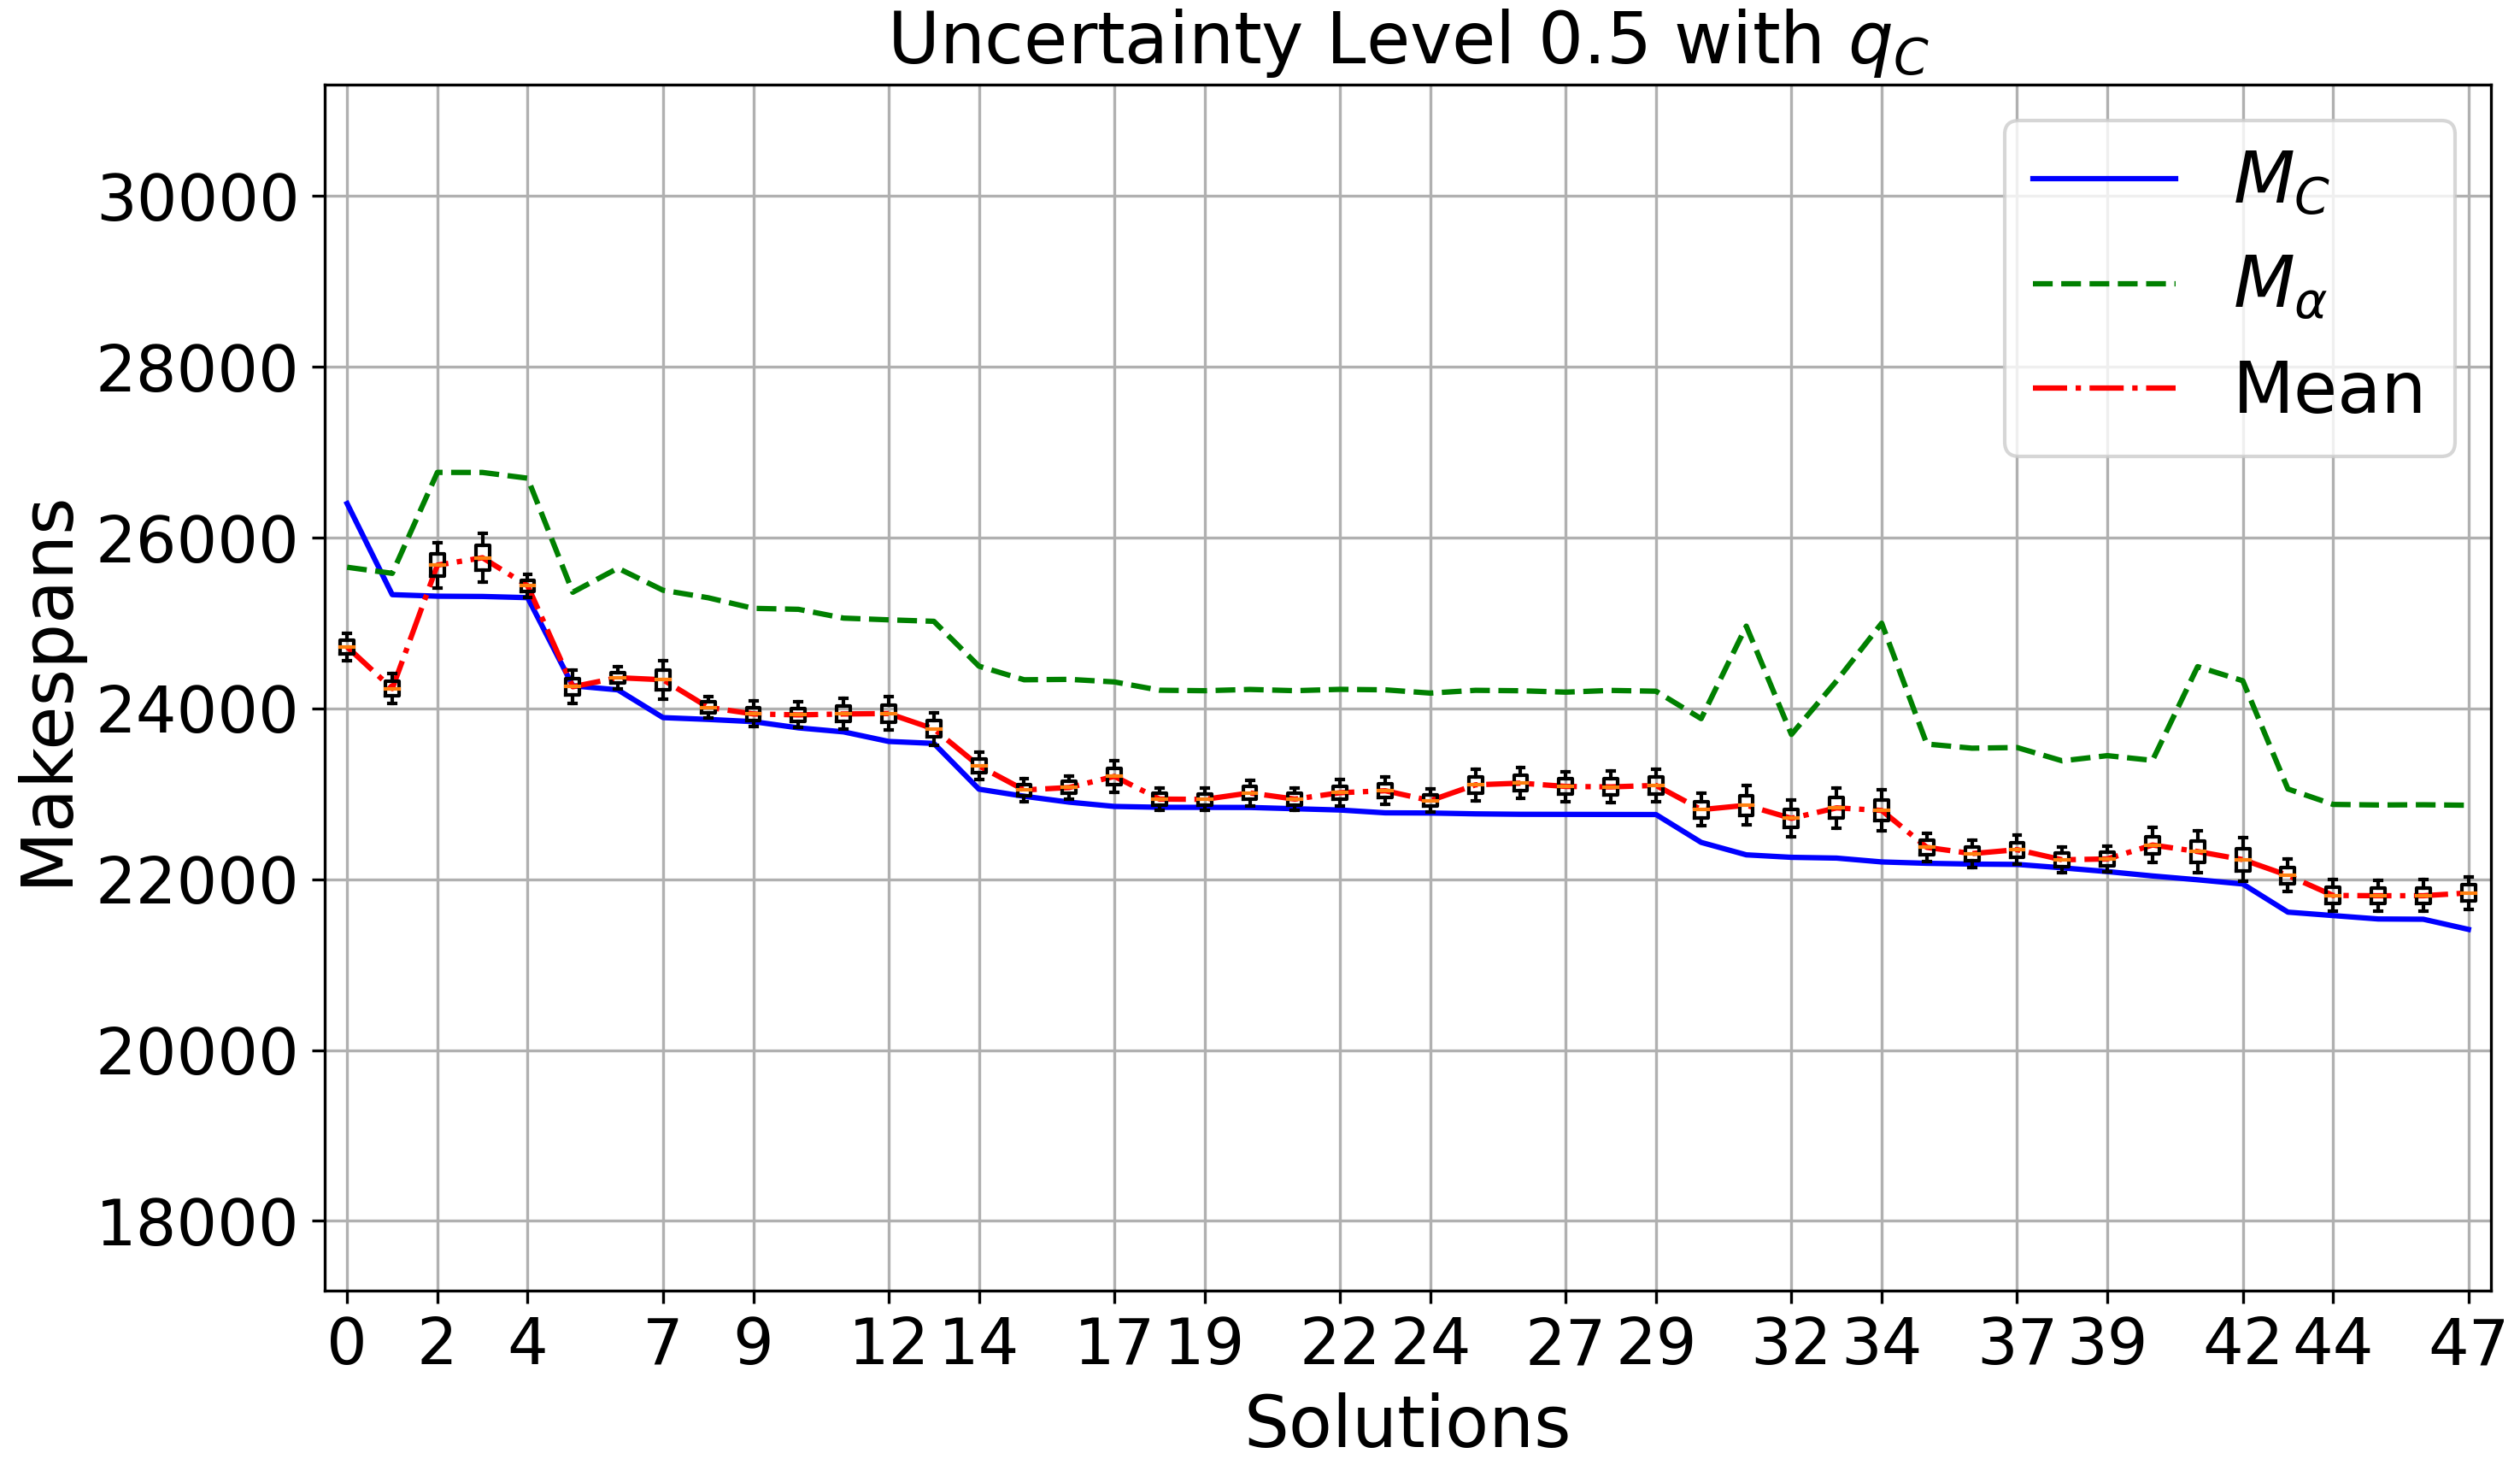
\includegraphics[width=0.47\textwidth]{images/uncertainty_caledars_2.png} }}%
    \caption{Comparison of all $M_C$ solutions returned by the CP solver, along with their corresponding $M_{\alpha}$ values and the \emph{Mean} computed over 1,000 simulations, for the synthetic \act{medium} problem with calendars and with an uncertainty level of $0.5$.}%
    \label{fig:comparison_qU_qC}%
\end{figure*}
 
In this section, we first outline the experimental settings, followed by a detailed description of the synthetic and real-world datasets used in our evaluation framework and their results. For synthetic experiments, we do not introduce other competitive methods, as the aim of these experiments is to test our framework under different uncertainty levels, problem sizes, and the presence or absence of resource calendars. For the real-world dataset, we do not compare our approach with other works due to their limitations, such as the absence of planned resource unavailability, the inability to account for uncertainty in activity durations, or scalability issues with large BPSP problems (see Section~\ref{sec:related}), which would lead to unfair comparisons.

\subsection{Experimental Setting}

\paragraph{Success Metrics} To assess the effectiveness of the proposed approach, we use two different metrics: the Normalized Probabilistic Makespan ($NPM$) and the Percentage of Improvement ($PI$). The $NPM$ evaluates the ratio between the minimum probabilistic Makespan ($M^*_{\alpha}$) and the minimum deterministic Makespan ($M^*_{C}$) obtained on synthetic experiments. It is computed as $NPM = M^*_{\alpha}/{M^*_{\text{C}}}$.

For the real-world dataset, we compute the $PI$ metric to measure the improvement between the $M^*_{\alpha}$ obtained from the optimized schedule and $M_{\text{act}}$ obtained from the actual schedule. It is calculated as $PI = ((M^*_{\alpha} - M_{\text{act}})/M_{\text{act}}) \times 100$.

\paragraph{Experimental Procedure} To transform the BPSP problems into deterministic ones, we need to define the $q$ value for each of them.
Instead of using $q_U$, we leverage the Monte Carlo simulation to obtain a more accurate estimation of the critical path compared to the one provided in the $q_U$ definition \eqref{eq:qU}.
%to the one used in 
To do that we employ \rims~\cite{MeneghelloFGR25}, a state-of-the-art business process simulator capable to accurately represent the complexity of business processes.
Specifically, we simulate the BPSP problem $1,000$ times using stochastic activity durations and identify the maximum critical path, $\pi$.
In this way, we obtain a deterministic Makespan that is closer to the probabilistic one, as we will show in Figure~\ref{fig:comparison_qU_qC}. This higher correlation between deterministic and stochastic Makespan allows us to accelerate the convergence to the minimal probabilistic Makespan $M_\alpha^*$.\footnote{In the repository \url{https://github.com/francescameneghello/IJCAI2025-Proactive-DataDriven-Scheduling-Business-Process} provides further evidence of the differences between applying $q_U$ and $q_C$. The latter allows finding $M^*_{\alpha}$ closer to $M^*_{\text{C}}$ and, within the same solver time limit, achieves a smaller $M^*_{\alpha}$ with fewer solutions, as shown in Figure~\ref{fig:comparison_qU_qC}. The downside is that using $q_C$, we cannot guarantee the lower bound property proved in Proposition~\ref{prop:lower}. }
%Instead of using $q_U$, which can be challenging to estimate due to the difficulty of determining the number of uncertain activities in the critical path---especially in BPSP problems that exhibit variability in case length and the number of resources involved---we estimate $q$ differently. Specifically, we simulate the BPSP problem $1,000$ times using stochastic activity durations and identify the maximum critical path, $\pi$. In this way, we can identify a deterministic Makespan closer to the probabilistic one as shown in Figure~\ref{fig:comparison_qU_qC}.\footnote{Our supplementary material provides further evidence of the differences between applying $q_U$ and $q_C$. The latter is not always a lower bound, but allows finding $M^*_{\alpha}$ closer to $M^*_{\text{C}}$.} 
The $q_C$ is then defined as follows~(\cite{beck2007proactive})
\[
q_C = \frac{\Phi^{-1}(1-\alpha)}{\sqrt{|\pi|}}\frac{\sqrt{Mean\{\sigma^2_{i,j}: A_i \in \pi\}}}{Mean\{\sigma^2_{i,j}: A_i \in \pi\}},
\] where $|\pi|$ is the number of activities in $\pi$.

%To retrieve $q_C$ and evaluate the solution, we use \rims~\cite{meneghello2023rimstool}, a state-of-the-art business process simulator capable of integrating predictive models to accurately represent the complexity of business processes.


After collecting all the solutions returned by the solver, we select the top $k$-solutions to be evaluated with \rims. These $k$-solutions are identified based on the last significant improvement\footnote{A significant improvement in the ordered list of deterministic solutions is defined as a $\Delta_i = (M_{\text{C}, j} - M_{\text{C}, i})/M_{\text{C}, j} \geq 0.20$ where solution $j$ precedes solution $i$.}, which tends to remain consistent in subsequent solutions. For instance, in Figure~\ref{fig:calendar_qC}, the last significant improvement is observed between solutions $42$ and $43$, marked by a notable step on the $M_{\text{C}}$ line, followed by a plateau. %extending until solution $47$. 

A 3-minute time limit is set for the CP solver, and the evaluation with \rims, thanks to the $k$-solution selection, takes an average of 5 minutes, with a maximum of 15 minutes for the largest problem in the DayHospital experiment. The experiments are conducted on a PC with 16 GB of RAM and an M2 processor.

\subsection{Synthetic Data Experiment} 

\paragraph{The Data} As synthetic data we use three problems from a set of publicly available JSP beanchmarks of different size \act{small} ($10 \times 10$), \act{medium} ($20 \times 20$), \act{big} ($50 \times 20$)~\cite{beanchmarks}\footnote{In the repository \url{https://github.com/francescameneghello/IJCAI2025-Proactive-DataDriven-Scheduling-Business-Process}, three other problems of different sizes are reported.}, where with $10 \times 10$ we indicate a problem with $10$ cases with $10$ activities for each case. For each of the problems, we set three levels of uncertainty $u \in \{0.1, 0.5, 1\}$ to define the standard deviation of each activity $a_{i,j}$ as a random number within the interval $\sigma_{i,j}= [0, u*\mu_{i,j}]$.
For each resource involved, we generate the corresponding calendars, assuming a working week of 5 days and 8 hours per day.

%Furthermore, we extend the synthetic data by generating three additional problems with the same structure, but activity durations depend on the type of case. The types represent three possible categories of patients in a hospital: the rare \act{red}, which leads to increased activity durations; \act{white}, which results in durations closer to the mean; and finally \act{yellow}, which falls in between the two.

\paragraph{Results} Table~\ref{tab:results_synthetic} presents the normalized probabilistic Makespans ($NPM$), showing that in the first set of experiments, the presence or absence of calendars does not significantly impact performance, except for the \act{Big} size at uncertainty levels $0.1$ and $1.0$. 
From an empirical analysis of the experiments with the presence of resource calendars, we note that a $q_C$ with respect to $q_U$ allows for representing activity durations closer to real times, enabling it to effectively leverage the planned availability and unavailability of resources to optimize the schedule.
Figure~\ref{fig:calendar_qC} shows that the average Makespans overlap with $M_C$, and $M_\alpha$ is slightly higher.  In contrast, $q_U$, as shown in Figure~\ref{fig:calendar_qU}, guarantees the lower bound (Section~\ref{sec:stoc_to_det}), but results in a worse solution compared to $q_C$.
Variance in $q$ may lead to a significant difference between the deterministic and the corresponding probabilistically minimal Makespans, even if their correlation remains. 
%This behavior appears more evident in the second set of experiments (see dark lines of Table~\ref{tab:results_synthetic}) where the $NPM$ metrics with calendars are always close to $1$ or slightly below. 


\subsection{DayHospital Experiment} 

\paragraph{The Data} In this experiment, we apply our approach to a real-world BPSP problem. Specifically, we use an entire year (2021) of data from DayHospital to learn the BPSP parameters and minimize the Makespan for the subsequent five months (January-May 2022), which serve as the test set.
The event log includes timestamped activities along with their designated resources as shown in Table~\ref{table:real_log_DT}. This allows us to identify the activities, the precedence relationships, and the resources, including their capacities and calendars, to define the BPSP problem.
Between 50 and 1,000 patients are treated every day in the hospital, depending on whether it is a weekday or a weekend, with over 1,600 activities taking place on the busiest days. 
To properly evaluate our approach, we compare the Makespan given from the simulation of the actual schedule and the $M^*_{\alpha}$ found with our approach.



\paragraph{Results}
Table~\ref{tab:results_hospital} reports the results achieved on the hospital dataset. We divided the days into \act{small}, \act{medium}, and \act{big} categories based on the number of activities treated in a day. For \act{medium} and \act{big} days, we observe, on average, a significant reduction in the global Makespan, up to 14\%, which corresponds to a reduction of approximately 4 hours. In the case of \act{small}, the scope for improvement is limited, yet we still observe improvements, even if at a slightly lower percentage. 




\begin{table}[tb]
    \centering
    \resizebox{.80\columnwidth}{!}{
    \begin{tabular}{c|cc|cc|cc}
        \toprule
        \textbf{Un. Level} & 0.1 & 0.1 & 0.5 & 0.5 & 1 & 1 \\
        \midrule
        \textbf{Calendar} & x & \checkmark & x & \checkmark & x & \checkmark \\
        \midrule \midrule
        \act{Small} &  1.00  &  1.00 & 1.03 & 1.00 & 1.13 & 1.13 \\
        \midrule
        \act{Medium} &  0.99  &  1.00 & 1.03 & 1.00 & 1.10 & 1.10 \\
        \midrule
        \act{Big} &  1.09  &  1.00 & 1.07 & 1.07 & 1.12 & 1.18 \\
        \bottomrule
    \end{tabular}
    }
    \caption{The NPM metrics are presented for each size, with and without the resource calendars.}
\label{tab:results_synthetic}
\end{table}


\begin{table}[tb]
    \centering
    \resizebox{.99\columnwidth}{!}{
    \begin{tabular}{l@{\hskip 0.05in}c@{\hskip 0.05in}c@{\hskip 0.05in}c@{\hskip 0.05in}c@{\hskip 0.05in}c@{\hskip 0.05in}c@{\hskip 0.05in}}
        \toprule
        \multirow{2}{*}{\textbf{Days}} & \textbf{Av.} & \textbf{Av. } & \textbf{Av.} & \textbf{Av.} & \textbf{Max} & \textbf{Av.} \\
         & \textbf{\#Cases} & \textbf{ \#Activities} & \textbf{ \#Resources} & \textbf{\% Imp.} & \textbf{\% Imp.} & \textbf{Imp.} \\
        \midrule
        \act{Small} &  98 &  136 & 33 & -1.2\% & -6\% & -14min \\
        \midrule
        \act{Medium} &  717  & 1242 & 237 & -4.8\% & -12\%& -69min \\
        \midrule
        \act{Big} &  848  & 1505 & 266  & -5.9\% & -14\% & -87min \\
        \bottomrule
    \end{tabular}
    }
    \caption{The days are divided into 3 groups based on 33rd and 67th percentiles.}
\label{tab:results_hospital}
\end{table}



\subsection{Discussion \& Limitations}

%Discuss the results, and interesting findings.
From the synthetic data evaluation, we verify the capability of our approach to optimize schedules for BPSP problems in the presence of various levels of uncertainty and planned resource unavailability. We define the $k$ selection allowing us to save time and achieve 
improved $M^*_\alpha$ of the problem. As for resource calendars, we observe the importance of selecting a $q_c$ that leads to producing $M^*_\alpha$  closer to the corresponding deterministic ones, thereby optimizing the utilization of available slots for the CP solver.
The DayHospital experiment shows promising performance despite
the limited clinical patient information available in the data (e.g., diagnosis, complexity, medical history). 
The use of RIMS~\cite{MeneghelloFGR25} can potentially leverage
%RIMS~\cite{MeneghelloFGR25} that we employ can potentially utilize 
such information to significantly improve the
estimation of activity durations.

%\footnote{{In the supplementary material, we present two additional experiments using predictive models: one for synthetic data with a generated patient attribute affecting activity durations, and another for real data, leveraging temporal features to fit durations.}

Below, we list several additional limitations of our work. As mentioned earlier, several simplified assumptions were necessary to apply process mining techniques and infer the BPSP problem from event logs. Additionally, comparisons with other methods addressing job duration uncertainty, if extended to incorporate planned resource unavailability, remain unexplored. Alternative job scheduling solvers could also be applied after defining the deterministic BPSP problem, leveraging the proposed Monte Carlo simulation to achieve the minimum probabilistic Makespan. Lastly, our approach focuses solely on minimizing the global Makespan, while resource-based objectives -- such as the minimization of costs or of idle resource times -- could better address organizational needs in BPSP problems.
\section{Related Work}
\label{sec:related}

\paragraph{Proactive and Data-Driven Scheduling}

%During the execution of real-world business processes, many random events occur, such as activities taking longer or shorter than expected due to various issues, and/or resources not being consistently available. 
%Therefore, it is necessary to account for the uncertainties when addressing the scheduling problem in business processes by using RCMPSP variants.


To the best of our knowledge, no other work combines together the unique features that characterize BPSP and that differentiate it from RCPSP, namely uncertain durations and resource unavailability.
Several papers have studied the uncertainty in job durations such as \cite{satic2022performance,liu2020multi,hauder2020resource,chen2019research,beck2007proactive,GomezBD23}; yet those works do not address resource unavailability.

In contrast, there are few papers on RCPSP constrained by resource time-window, mainly for human resources with working time constraints, resources with planned maintenance attributes~\cite{ding2023extensions} or resource calendars \cite{kreter2018mixed}. \cite{tian2018optimizing} address resource unavailability planning by defining randomly generated periods during which certain resources are unavailable. However, these works do not address duration uncertainty.
%Indeed, there are few papers on RCPSP/RCPSP constrained by resource time-window, mainly for human resources with working time constraints, resources with planned maintenance attributes, and renting resources \cite{ding2023extensions}. \cite{kreter2018mixed} introduced the resource calendar to describe the unavailability of resources in the study of resource availability costs, but does not address job duration uncertainty as in the works of \cite{yang2020multi,winklehner2022flexible}.

%Business processes are also characterized by variability in project paths, which many approaches, such as \cite{satic2022performance,tian2018optimizing}, cannot handle due to computational intractability. The basic relationship between jobs in the RCMSPS is the end-start relationship, which establishes that a job cannot begin execution until all its predecessor jobs have been fully completed. Meanwhile, in business processes, some jobs can be executed simultaneously, as addressed in \cite{tian2018optimizing}.
%\cite{senderovich2019learning,vcapek2012production} works overcome the problem of handling a large number of project variants by also considering the possibility of concurrent job execution using a particular Petri net structure; however, they do not account for the stochastic nature of durations and resources.
%\cite{tian2018optimizing} address resource unavailability planning by defining randomly generated periods during which certain resources are unavailable. 

Lastly,  the majority of studies test their solutions using generated instances, while only a small portion, about 11\%, utilize real-world-based instances \cite{sanchez2023survey}. 
The only exception is the work of \cite{senderovich2019learning}.
Our approach extends \cite{senderovich2019learning} by incorporating stochastic activity
durations, as well as by discovering duration distributions and resource calendars from event data. 

\paragraph{Resource Allocation in Process Mining}

Several works in process mining have addressed the problem of resource allocation, which aims to ensure that each activity in a process case is executed at the right time and with the right resources \cite{Kumar_2002}.
Much of the research in this area focuses on online resource allocation, involving reactive scheduling where tasks are dynamically assigned to resources at runtime. These strategies are particularly useful in settings where information becomes available over time, such as the appearance of unexpected cases or unforeseen resource unavailability. Various techniques have been proposed to address these problems, including batch allocation strategies \cite{Delias_2011,Arias2018HumanRA,Zeng_2005}, predictive allocation \cite{Park_2019}, reinforcement learning approaches \cite{HUANG2011127,Zbikowski_2023,MIDDELHUIS2025102492,BEEREPOOT2023103837,Meneghello_2024}, as well as formulations based on assignment problems or parallel machine scheduling \cite{Kunkler_2024}.

Fewer works have explored offline scheduling, where an initial schedule or roster is required from the outset. For instance, in \cite{Havur_2022}, the problem is formalized as an Answer Set Programming (ASP) formulation, enabling an ASP solver to compute a schedule. Similarly, \cite{Aalst_1996,DOERNER20061798} use a Petri net formalization of control flow and resource perspectives, solving the problem through the reachability graph. Notably, only \cite{DOERNER20061798} considers stochasticity in activity durations. These approaches lack mechanisms to ensure schedule robustness under temporal fluctuations. In this context, \cite{DiCunzolo_2024} is the only work that integrates operations research with PPM predictive models to produce robust schedules.
Despite these advances, none of the existing methods considers planned resource unavailabilities in a proactive setting.






\section{Conclusion}
\label{sec:conclusion}

In this work, we introduced the Business Process Scheduling Problem (BPSP) to address the challenges of scheduling business processes with stochastic activity durations and planned resource unavailability. Our solution framework combines process mining for parameter inference, deterministic transformations for uncertainty modeling, constraint programming for robust scheduling, and Monte Carlo simulation for probabilistic evaluation. Through evaluation on synthetic datasets, we demonstrated the adaptability of our solution to varying uncertainty levels, problem sizes, and resource configurations, achieving effective optimization of the probabilistic Makespan. Real-world validation on hospital data showcased the utility of the approach, achieving up to 14\% reductions in global Makespan.

Future work will focus on addressing the limitations identified in this study. Enhancing the scalability of the framework to handle larger, more complex business processes and integrating adaptive real-time rescheduling capabilities will extend its applicability to realistic environments. Exploring multi-objective optimization to balance trade-offs such as cost, resource utilization, and Makespan could further align the framework with organizational goals when scheduling business processes. Additionally, refining parameter inference methods to handle incomplete or noisy event logs and incorporating contextual data would significantly improve the practicality of the approach across diverse domains.
Lastly, while we currently use Monte Carlo simulation to handle uncertainty by sampling from the full distribution of activity durations, we aim to explore stochastic programming in future work. Stochastic programming offers a more structured approach by optimizing over a finite set of scenarios with assigned probabilities, potentially reducing uncertainty more effectively. However, its main limitation lies in the need to predefine a manageable set of scenarios, which is impractical in our case due to the vast number of possible realizations. As we introduce new uncertainties—such as variability in activity sequences—scenario-based methods may become more tractable, making stochastic programming a promising direction for future exploration.


\subsubsection{Acknowledgements}
We acknowledge the support of the PNRR project FAIR - Future AI Research (PE00000013), under the NRRP MUR program funded by the NextGenerationEU, the HORIZON 2020 HumanE-AI project (Grant 952026), and the PRIN project PINPOINT Prot. 2020FNEB27, CUP H23C22000280006 and H45E2100021000. 

% The file named.bst is a bibliography style file for BibTeX 0.99c
\bibliographystyle{named}
\bibliography{ijcai25}

%\clearpage

%\input{sections/supplementary_material}

\end{document}

